\section{The USB Interface and the Host Tools}
\label{sec:host}

The board is the station; what crosses USB is messages and control, at
a few hundred bytes per second.  This section covers that seam and
everything built on the host side of it: the modem as a USB device and
the wire protocol it speaks (specified in full in
\texttt{docs/usb-protocol.md} and \texttt{docs/modem-protocol.md}), the
host driver and the timing rules the boards imposed on it, the
demonstration infrastructure, the interface documents, and two
applications that put existing packet-radio software on the link --- a
KISS TNC and an IP tunnel --- each of which found a defect in whoever
owned the timers.

\subsection{The Modem as a USB Device}
\label{sec:cport_usb}

A modem that reaches the PC over a USB-to-serial bridge appears as one
more \texttt{/dev/ttyACM*} among however many adapters are attached,
numbered by enumeration order --- so the host has to guess which port is
the modem, and guesses wrong after a reboot or a re-plug. The C port
therefore presents the STM32's own USB peripheral as a device with an
\emph{identity}: a vendor-specific interface (class \texttt{0xFF}, so no
operating system binds a driver of its own), two bulk endpoints, a fixed
VID:PID, and a serial string that is the part's 96-bit unique ID. Two
modems on one host are then always distinguishable, and a udev rule
gives each unit a stable \texttt{/dev/ofdm-modem-<serial>}. The wire
format is length-prefixed frames behind two sync bytes and carries no
checksum, because USB already CRCs and retries every packet; the
parser's resynchronisation count is therefore a fault counter rather
than a statistic, and it read zero throughout everything below.

The protocol codec is deliberately free of any USB, station or platform
dependency --- bytes in, frames out --- so one implementation serves the
firmware, the host driver, and an \emph{emulator} that runs the real
device-side C over a pipe. The host driver was tested against that
emulator (11 checks, plus 18 on the codec itself, and 40\,MB of random
input under the sanitizers) before any hardware was involved, which is
what made the hardware phase a search for hardware problems only.

\paragraph{Bring-up.} TinyUSB's dwc2 port drives the H743's
\texttt{USB2\_OTG\_FS} core; the image runs from RAM over the JTAG probe
of Section~\ref{sec:cport_ontarget}, with a progress beacon at a fixed
DTCM address, so the board's flash is never written. Figure~\ref{fig:usbenum}
shows enumeration. Three things cost real time, and all three present as
something other than what they are:

\begin{itemize}
    \item \textbf{The USB supply has two sources needing opposite
          settings.} A board feeding \texttt{VDD33USB} from its own
          3.3\,V rail wants \texttt{USB33DEN} alone; one deriving it
          from VBUS also wants \texttt{USBREGEN}. Enabling the regulator
          on the first kind holds \texttt{USB33RDY} low forever:
          \texttt{PWR\_CR3} read \texttt{0x03000042}, then
          \texttt{0x05000042} the instant \texttt{USBREGEN} was cleared.
          The firmware now tries the external supply first and falls
          back, recording which worked. It also no longer spins on the
          flag: an unbounded wait there hung before anything could
          report why, and looked exactly like a crash.
    \item \textbf{A USB-C-to-C cable does not work on most development
          boards.} They omit the CC pull-down resistors that mark the
          board as a device, so a C-to-C host never detects an attach
          and never sources VBUS --- every register on the device reads
          correct and nothing appears on the bus. A C-to-A cable needs no
          CC negotiation.
    \item \textbf{A RAM-resident image has no vector table.} With VTOR
          still pointing at the resident firmware, the first USB
          interrupt --- and any fault --- vectored into another program's
          handler and vanished. The image now installs its own table;
          within a minute it caught an unhandled SysTick nobody had
          switched off (\texttt{ICSR} \texttt{0x80F}, \texttt{CFSR} and
          \texttt{HFSR} zero). Genuine faults stop and report; unexpected
          interrupts are masked, counted and survived.
\end{itemize}

\begin{figure}[H]
    \centering
    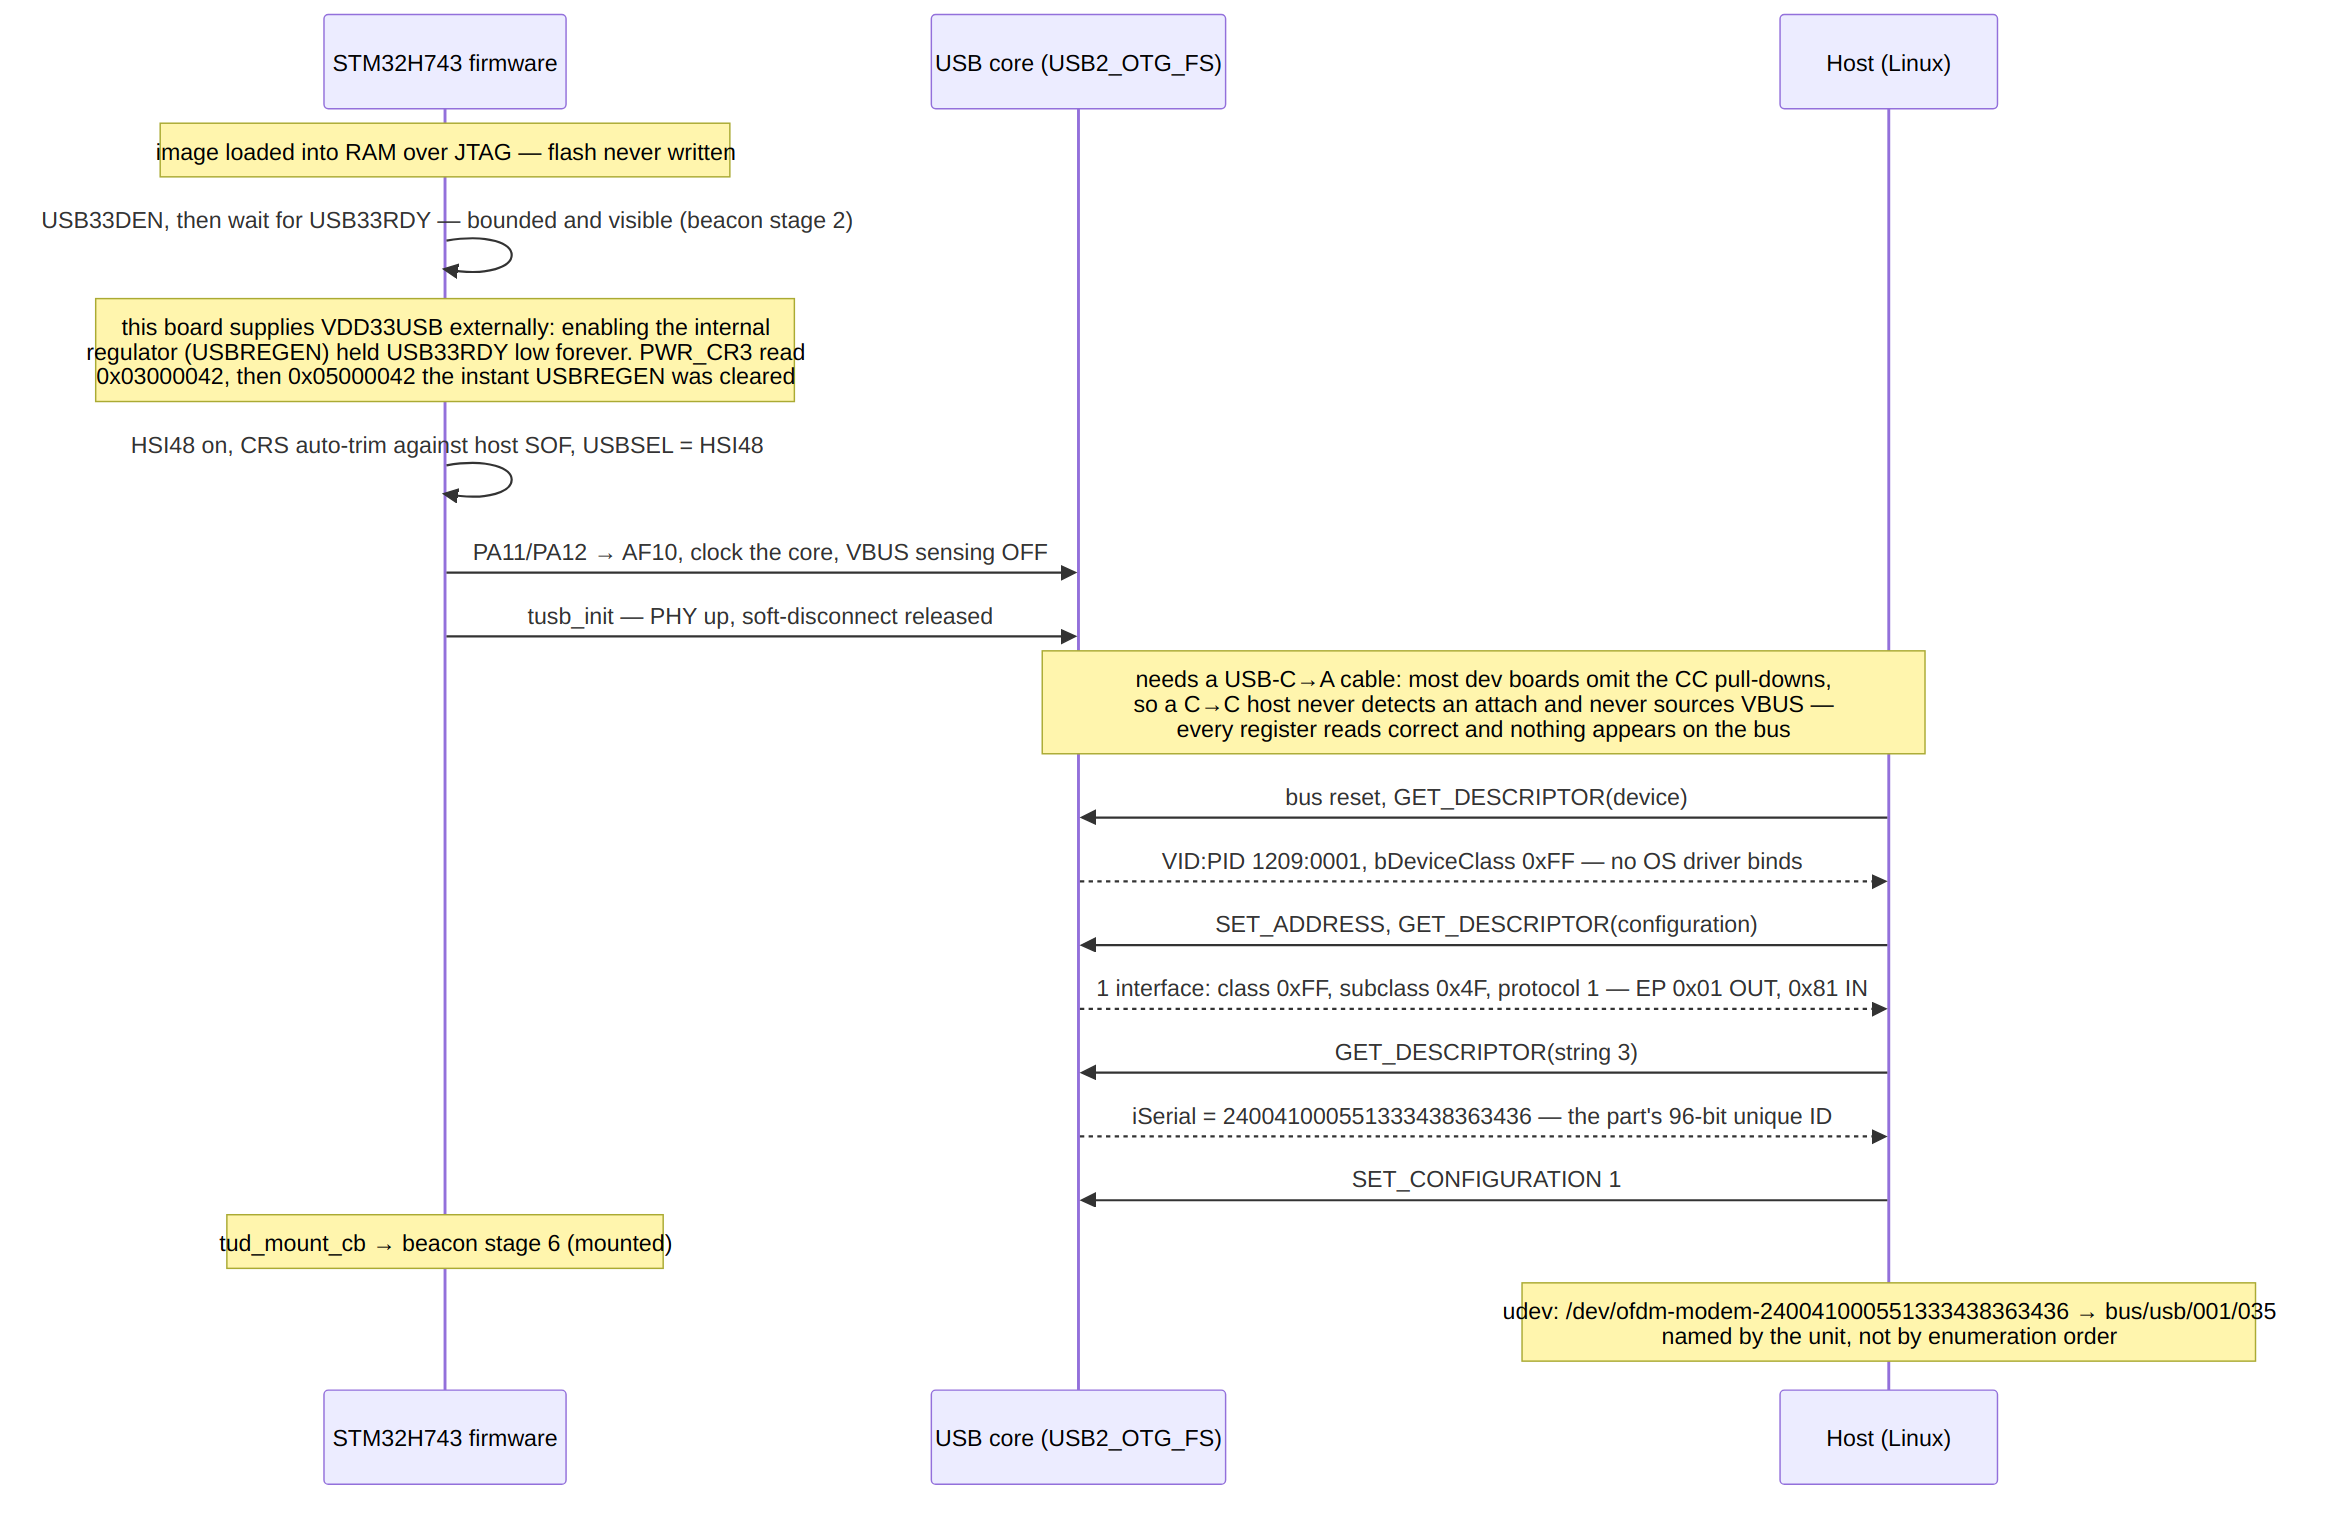
\includegraphics[width=0.92\textwidth]{images/usb_enum_seq.png}
    \caption{Enumeration: supply detection, clocks from HSI48 (trimmed
             against the host's SOF, so the firmware is correct whatever
             the board's crystal), and the descriptors that give the
             device its identity.}
    \label{fig:usbenum}
\end{figure}

\paragraph{A session.} Figure~\ref{fig:usbsession} traces a host
session against the real link layer: the station's queues, rate ladder
and reply timers run for real behind the endpoints, with a stub PHY that
accounts air time and transmits nothing --- the honest shape of a modem
with its antenna disconnected. Status is pushed unprompted twice a
second whenever the device is mounted; the diagnostic event stream is
opt-in and yields to everything else, because a lost diagnostic costs
nothing and a lost reply costs the session.

\begin{figure}[htbp]
    \centering
    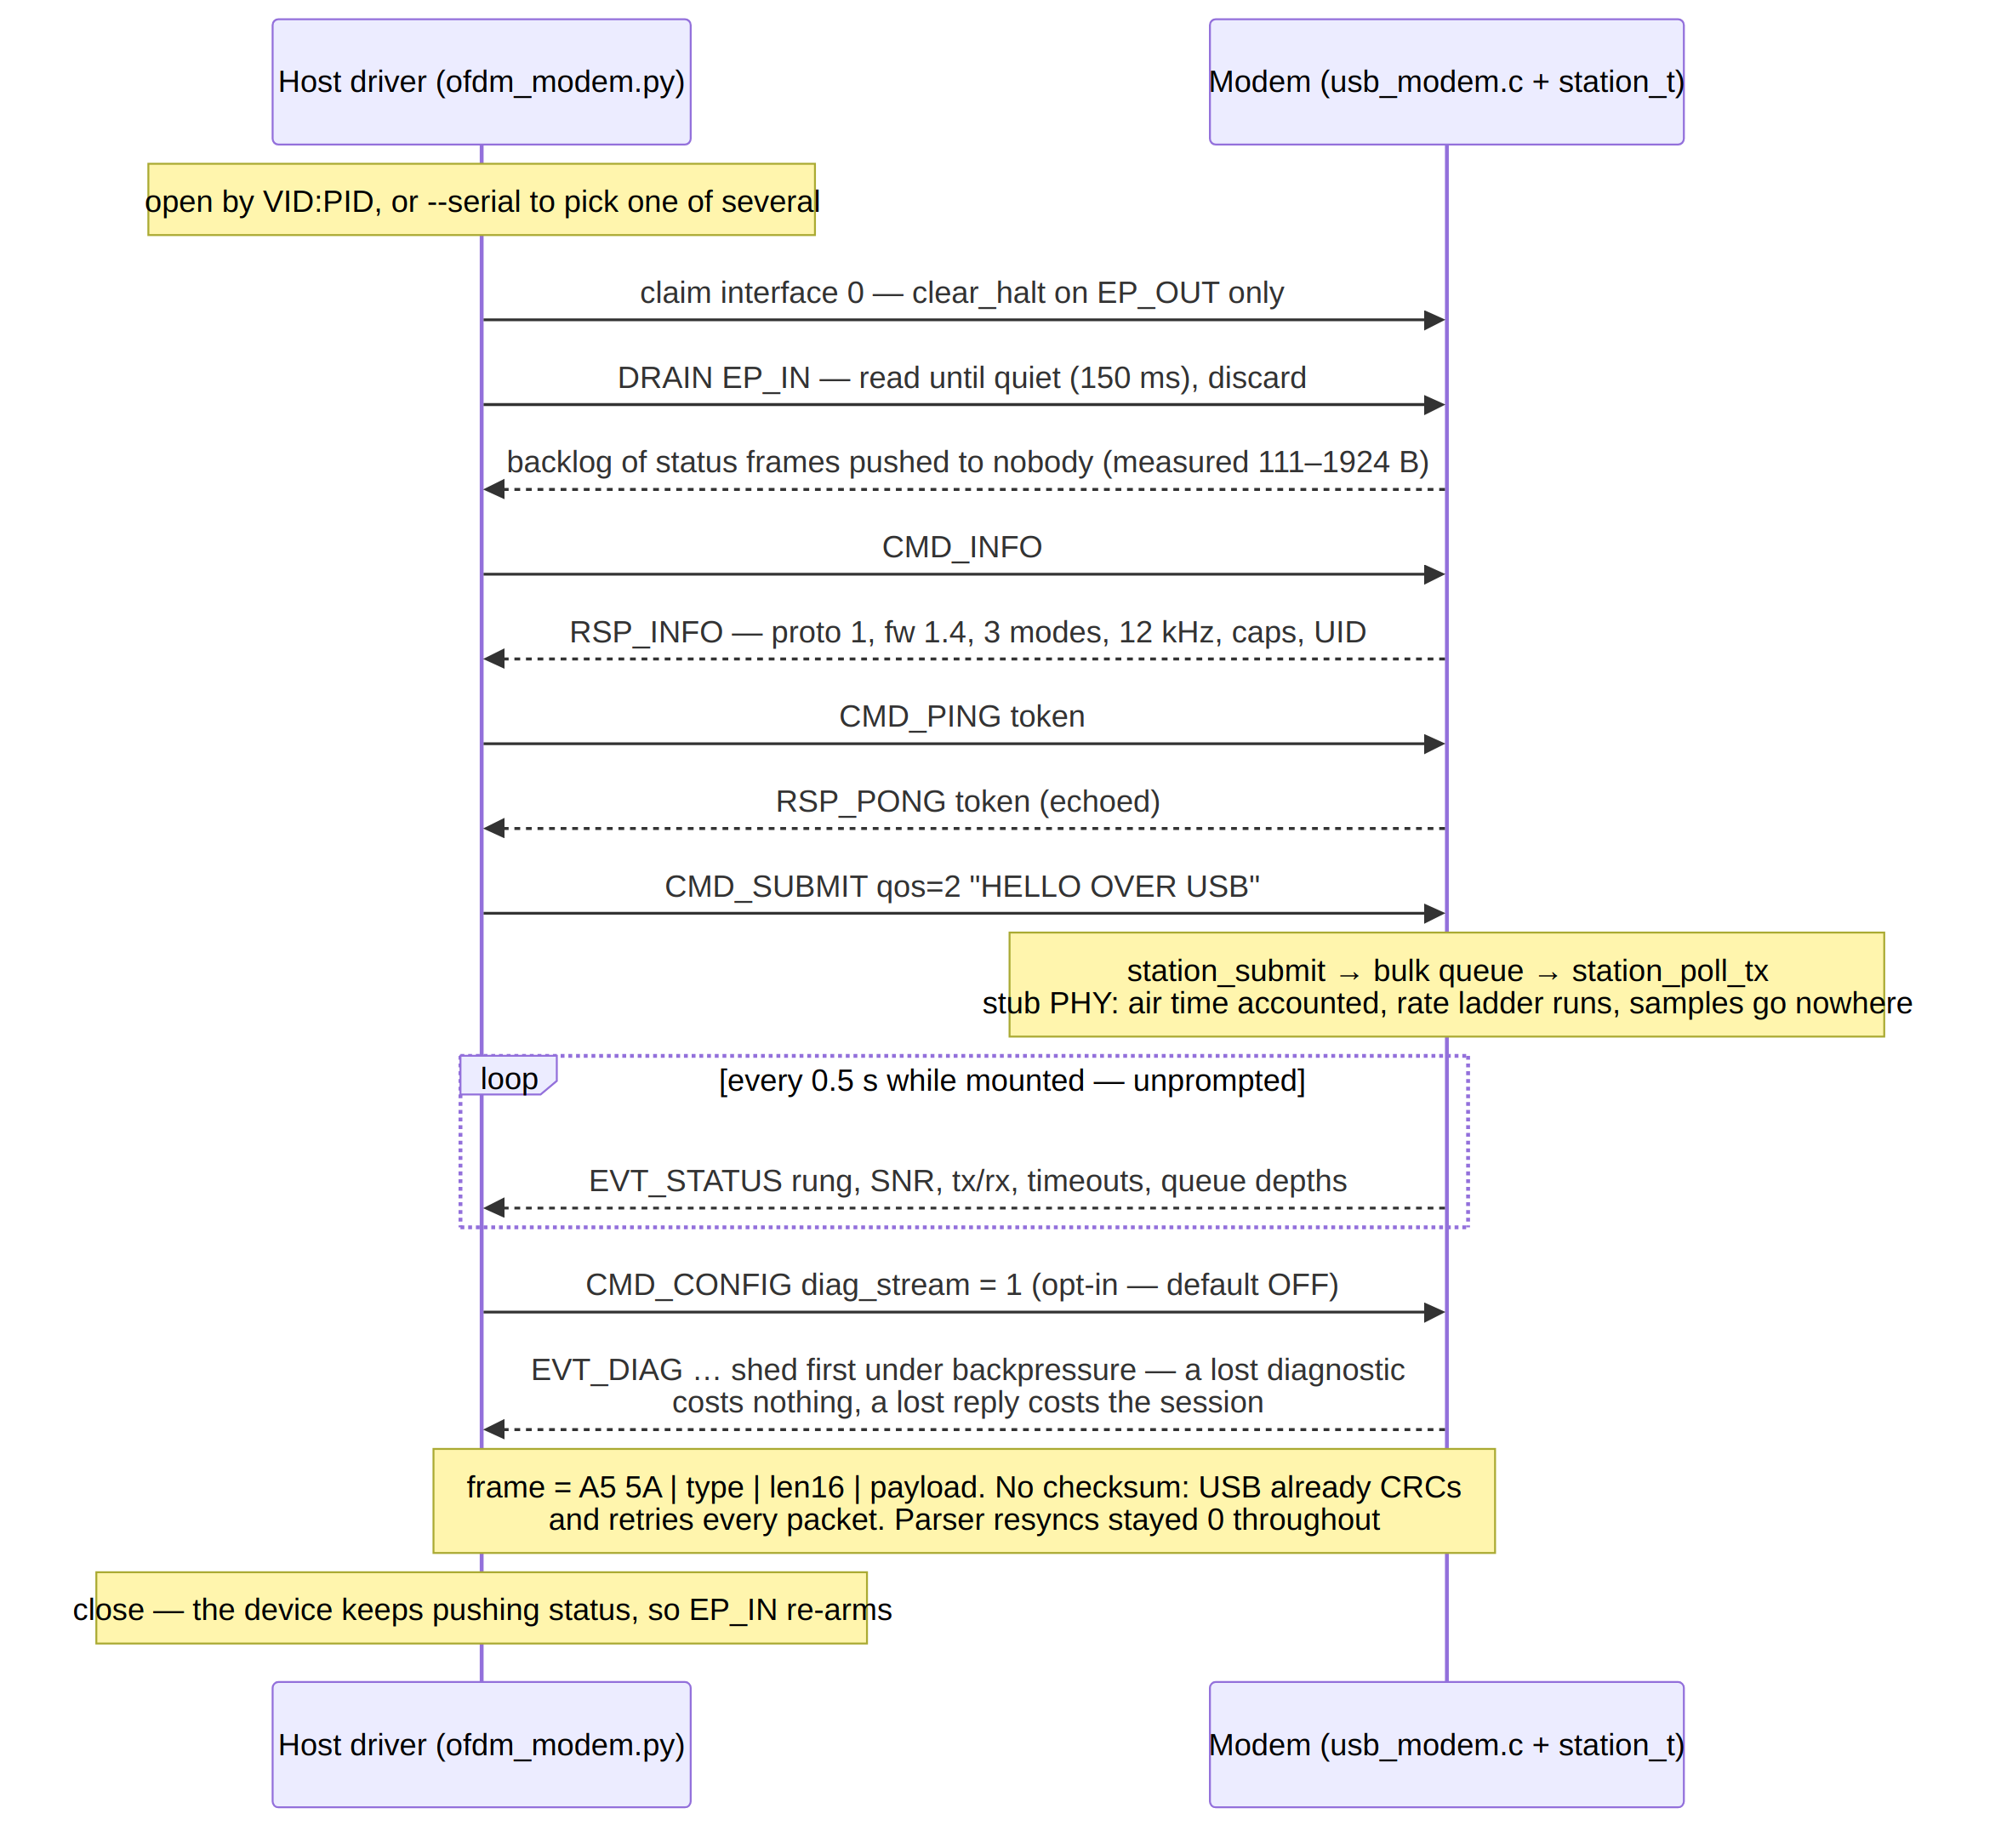
\includegraphics[width=0.92\textwidth]{images/usb_session_seq.png}
    \caption{A host session: open, drain, identify, command and reply,
             unprompted status, opt-in diagnostics.}
    \label{fig:usbsession}
\end{figure}

\paragraph{The wedge, and why the host must drain rather than reset.}
The station image enumerated correctly and then, for most of a day,
answered nothing and fell silent after a single packet --- deterministically,
across four builds. Five hypotheses were disproven by measurement
(a diagnostic firehose, loop starvation under polling, cache against
DMA, polling against interrupts, the clock), and three unrelated bugs
fixed on the way, before the instrumentation at the moment of the stall
read: staging queue empty, 150 bytes free of a 512-byte TinyUSB transmit
FIFO, 399 bytes handed over. That is 362 bytes sitting \emph{inside}
TinyUSB unsent --- 29 (the \texttt{RSP\_INFO} reply) plus nine 37-byte
status frames, exactly --- and $399-362=37$: precisely one frame ever
reached the wire. The device was not silent; it was mute.

The cause, confirmed from TinyUSB's source and shown in
Figure~\ref{fig:usbreopen}, is an interaction between an ordinary host
habit and the library's clear-stall handling. Because the device pushes
status unprompted, its IN endpoint is normally \emph{armed} with a frame
when a host opens it. The host driver called \texttt{clear\_halt} on
that endpoint on open --- a common recovery idiom, and one added during
this work. \texttt{usbd\_edpt\_clear\_stall} drops its software BUSY
flag unconditionally (its own comment calls this ``long-standing
behavior''), while the dwc2 \texttt{dcd\_edpt\_clear\_stall} only clears
the STALL bit and resets the PID; nothing disarms the hardware. The next
flush sees ``not busy'' and re-arms the endpoint on top of a live
transfer --- undefined on the core --- so one packet escapes, the
completion no longer matches what the library started, and BUSY never
clears. The level-triggered FIFO-empty interrupt then storms:
\texttt{isr\_count} reached 90 million.

It was confirmed by prediction rather than by fix. Holding status frames
until the host had spoken, so the endpoint was idle at open, made the
\emph{first} open work --- and every later open still wedged, exactly as
the mechanism requires, since by then the device was pushing again.

The fix is on the host: consume the armed transfer instead of resetting
the endpoint. The driver reads the IN endpoint with short timeouts until
it goes quiet and discards what it finds; \texttt{clear\_halt} is kept
for the OUT endpoint only, where three opens against an armed endpoint
measured harmless. The device is unchanged --- pushing status while
mounted is the right thing for a modem to do, and is the case a driver
must handle. Verified on the part: three consecutive opens (draining
1924, 185 and 111 stale bytes) and a session killed mid-read then
reopened (draining 37 bytes: the one frame armed at the kill), all
answering, submitting and reading with zero resynchronisations;
\texttt{isr\_count} 293 against 90 million wedged, no faults, no drops.

\begin{figure}[htbp]
    \centering
    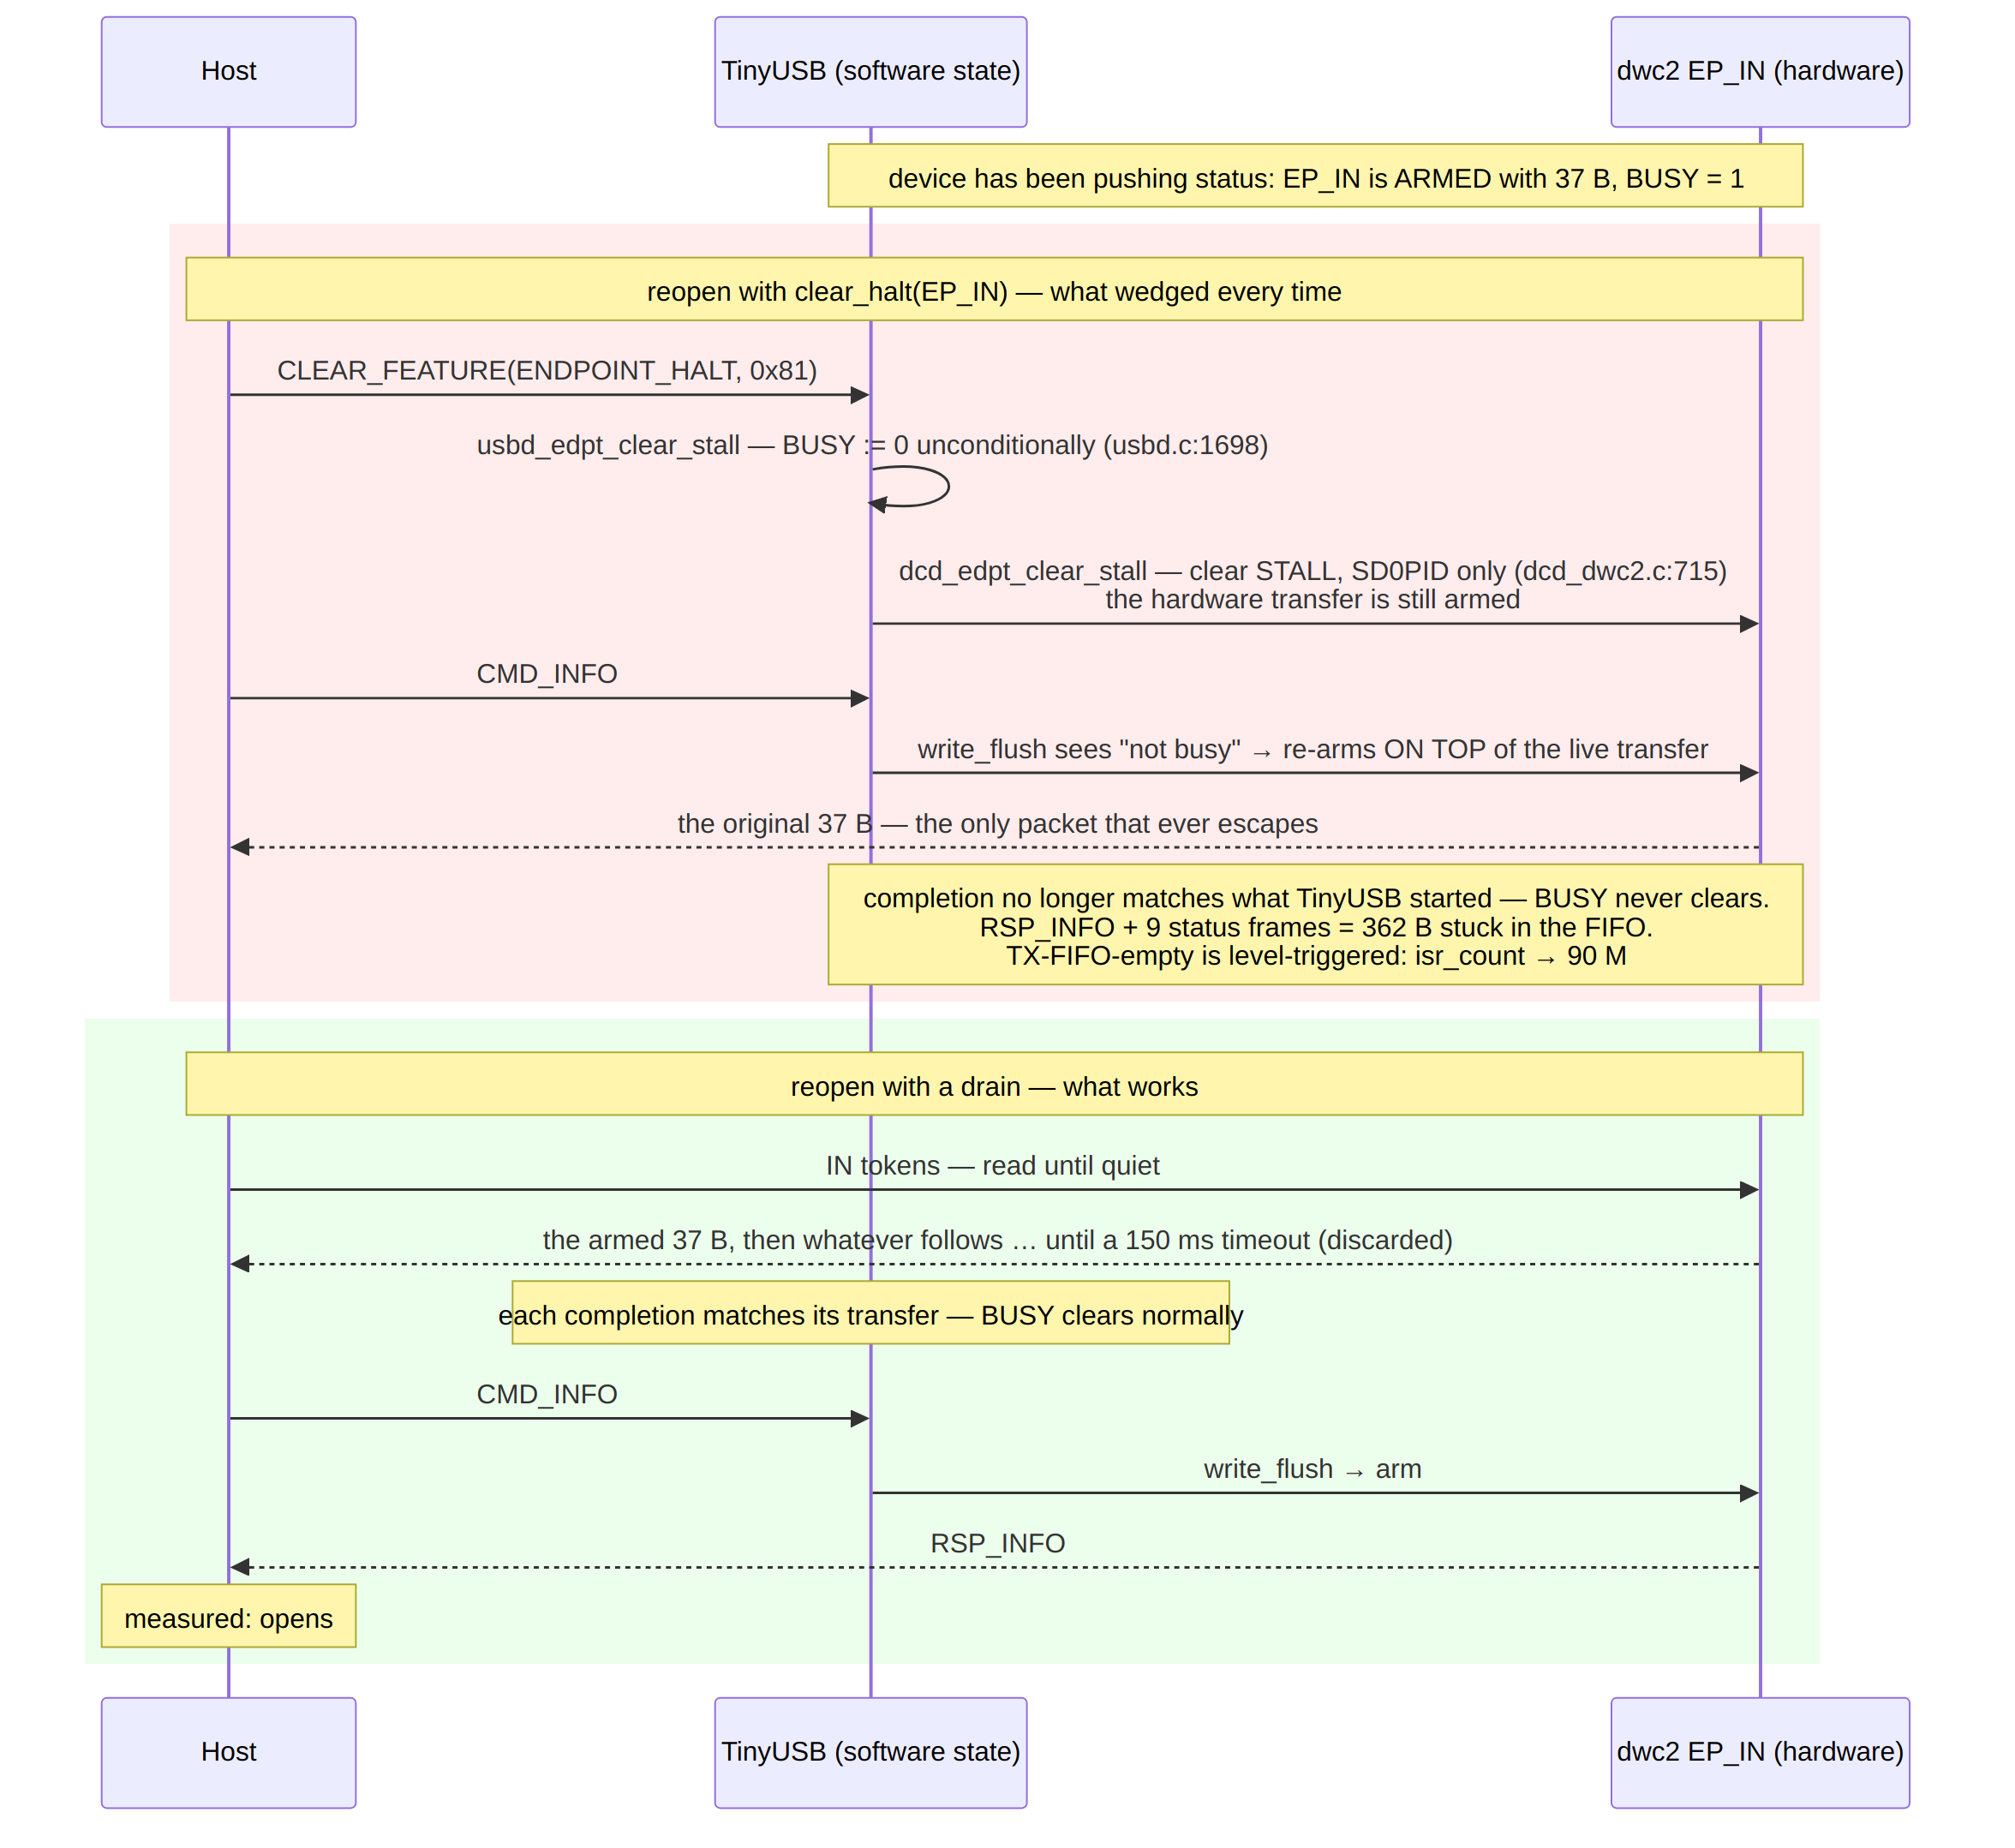
\includegraphics[width=0.92\textwidth]{images/usb_reopen_seq.png}
    \caption{Reopening against a device that is already pushing. Above:
             \texttt{clear\_halt} on an armed IN endpoint desynchronises
             TinyUSB's software state from the hardware and wedges it
             after one packet. Below: draining the endpoint consumes the
             armed transfer through the normal path.}
    \label{fig:usbreopen}
\end{figure}

Two qualifications. VID:PID \texttt{1209:0001} is the pid.codes
\emph{test} identifier, correct for development and wrong for anything
shipped: a released unit needs an allocated product ID, or it collides
with every other prototype using the same one. And the device has not
been made robust to \texttt{clear\_halt} on an armed endpoint itself;
that is TinyUSB's clear-stall path rather than this project's, so the
contract is stated instead --- any client for this device must drain,
not reset.

\subsubsection{The host side, and the 2.3-second stall}
\label{sec:cport_hosttiming}

The drain-not-reset rule above is one instance of a wider mistake, and
the rest of it surfaced only once the boards were doing real work.  A
host naturally assumes the device is always ready to talk.  This one is
not: a single \texttt{rxs\_push} can occupy the processor for
2283\,ms at the end-of-frame commit (Section~\ref{sec:cport_radio}, the
same measurement that sizes the capture FIFO), and for that whole
window USB is simply not serviced.  Every host-side defect found after
the two-board stand came up is a deadline shorter than that number.

\begin{table}[H]
    \centering
    \caption{Host timeouts against the device's worst blocking decode.
             Each was chosen before that figure was measured, and each
             failed in a way that looked like something else.}
    \label{tab:host_timeouts}
    \small
    \begin{tabular}{@{}lllp{4.6cm}@{}}
    \toprule
    \textbf{Operation} & \textbf{Was} & \textbf{Now} &
    \textbf{Symptom} \\
    \midrule
    Bulk write, Python & 1000\,ms & 5000\,ms &
    console died mid-transfer with a traceback out of its 1\,Hz
    heartbeat \\
    Bulk write, C & 2000\,ms & 5000\,ms &
    ``usb write failed'', frame lost \\
    Serial string, C & $4\times50$\,ms & $10\times300$\,ms &
    intermittent \texttt{<unreadable>} in \texttt{--list} \\
    Serial string, Python & none & $10\times300$\,ms &
    \texttt{ValueError: no langid}, 3 opens in 12 \\
    \bottomrule
    \end{tabular}
\end{table}

The last of those is worth more than its size, because the obvious fix
did not work.  Adding retries left the \emph{first} open in twelve
still failing, and failing in 3.7\,s --- which is 3.7\,s of not
touching the bus, because pyusb caches a failed language-ID fetch as an
empty tuple and every subsequent string request then raises
immediately, forever, on that device object.  A retry that does not
clear the cache is decoration.  With the cache reset between attempts:
60 opens of both boards, no failures, and a cold open after fifteen
idle minutes --- the reported case --- takes 0.17\,s.  The
distinguishing evidence was the shape of the failure rather than its
message: the \emph{first} open failed and the next eleven succeeded in
0.16\,s each, which is a cache being poisoned, not a bus being busy.
The error text says ``permission issue'', and it is not one.

Two further host defects were not about timing at all, and both are the
same shape as the sentinel family of Section~\ref{sec:cport_sentinel}:
a value that had drifted from its definition.  The Python host's
maximum frame size was still 1024\,bytes, the protocol's original,
while \texttt{UP\_MAX\_PAYLOAD} had grown to 3336 for whole-message
transfers --- so its parser discarded every frame declaring more, and
the Python console received small traffic perfectly while file parts
vanished, from a board that had decoded and acknowledged them.  And
\texttt{pyusb} was never in \texttt{requirements.txt}, only in a README
line, so the environment the project is normally run from could not
talk to a board at all.  Both are now pinned by tests
(\texttt{host/test\_modem.py}), which is the only thing that keeps a
constant duplicated across two languages honest.

\subsection{Demonstration Infrastructure}
\label{sec:cport_demo}

The C stack runs end-to-end in an interactive demonstration
(\texttt{demoapp/}): a virtual channel daemon exposes two station
devices and a configuration device over Unix sockets, moves 12\,kHz
\texttt{int16} audio in paced ticks, and applies propagation delay,
AWGN sized against the delivered-signal RMS, one-pole Rayleigh fading,
and half-duplex muting; an optional audio mode plays each station's
receive signal on one stereo channel with the sound card as the pacing
clock, making the protocol audible (the EXTREME bootstrap's 21-second
warble adapting up to sub-second QAM16 chirps).  Two console station
applications (three streaming receivers each, one per mode, over the
shared ring) provide messaging, multi-part file transfer over the
burst protocol, channel statistics, the diagnostic event stream, and
the oscillator fine-tune command.  A scripted smoke test drives the
whole stack --- text plus a 5\,000-byte file across the impaired
channel, byte-compared on arrival --- at $25\times$ time scale; the
protocol clocks itself from received samples, so behaviour is
identical at any scale.  The stop-and-wait inefficiency, the burst
protocol's window bugs, the carrier-sense threshold and the rung-0
fallback were all found by this infrastructure rather than by
inspection.

Figure~\ref{fig:sendfileseq} traces a file transfer through it.  Two
decisions in that sequence are worth isolating.

The file is deflated \emph{whole} before being split into parts, not
per part: a 14162-byte configuration file becomes 5015 bytes on air
($2.82\times$), and compressing each 3\,kB part separately would throw
most of that away.  Compression lives in the application rather than in
\texttt{cport/}, which keeps the C port dependency-free --- an MCU
build swaps zlib for miniz or heatshrink and the wire format is plain
\textsc{deflate} either way.

The transfer also \emph{negotiates before it commits}.  The transmit
rung decays by one step per 90\,s of peer silence
(Section~\ref{sec:link}), so a transfer started after a quiet
spell would otherwise open at a rung the link has never been tested at:
measured, a 37.0\,s frame at rung~4 immediately before the next
exchange settled at rung~12 and 5.1\,s.  A sub-second control frame is
answered, and an answered frame is what moves the ladder, so the probe
goes first and the bulk queue follows behind it.  The staleness test
must ask whether the peer has \emph{ever} reported rather than
subtracting from the initial timestamp --- the sentinel is
$-10^{9}$, and doing the arithmetic anyway reported that the peer had
last been heard from 1000000058\,seconds ago.  It is the same rule the
link layer already follows for sequence numbers, where every value
0--7 is legitimate and ``nothing yet'' must be its own state.

\begin{figure}[H]
    \centering
    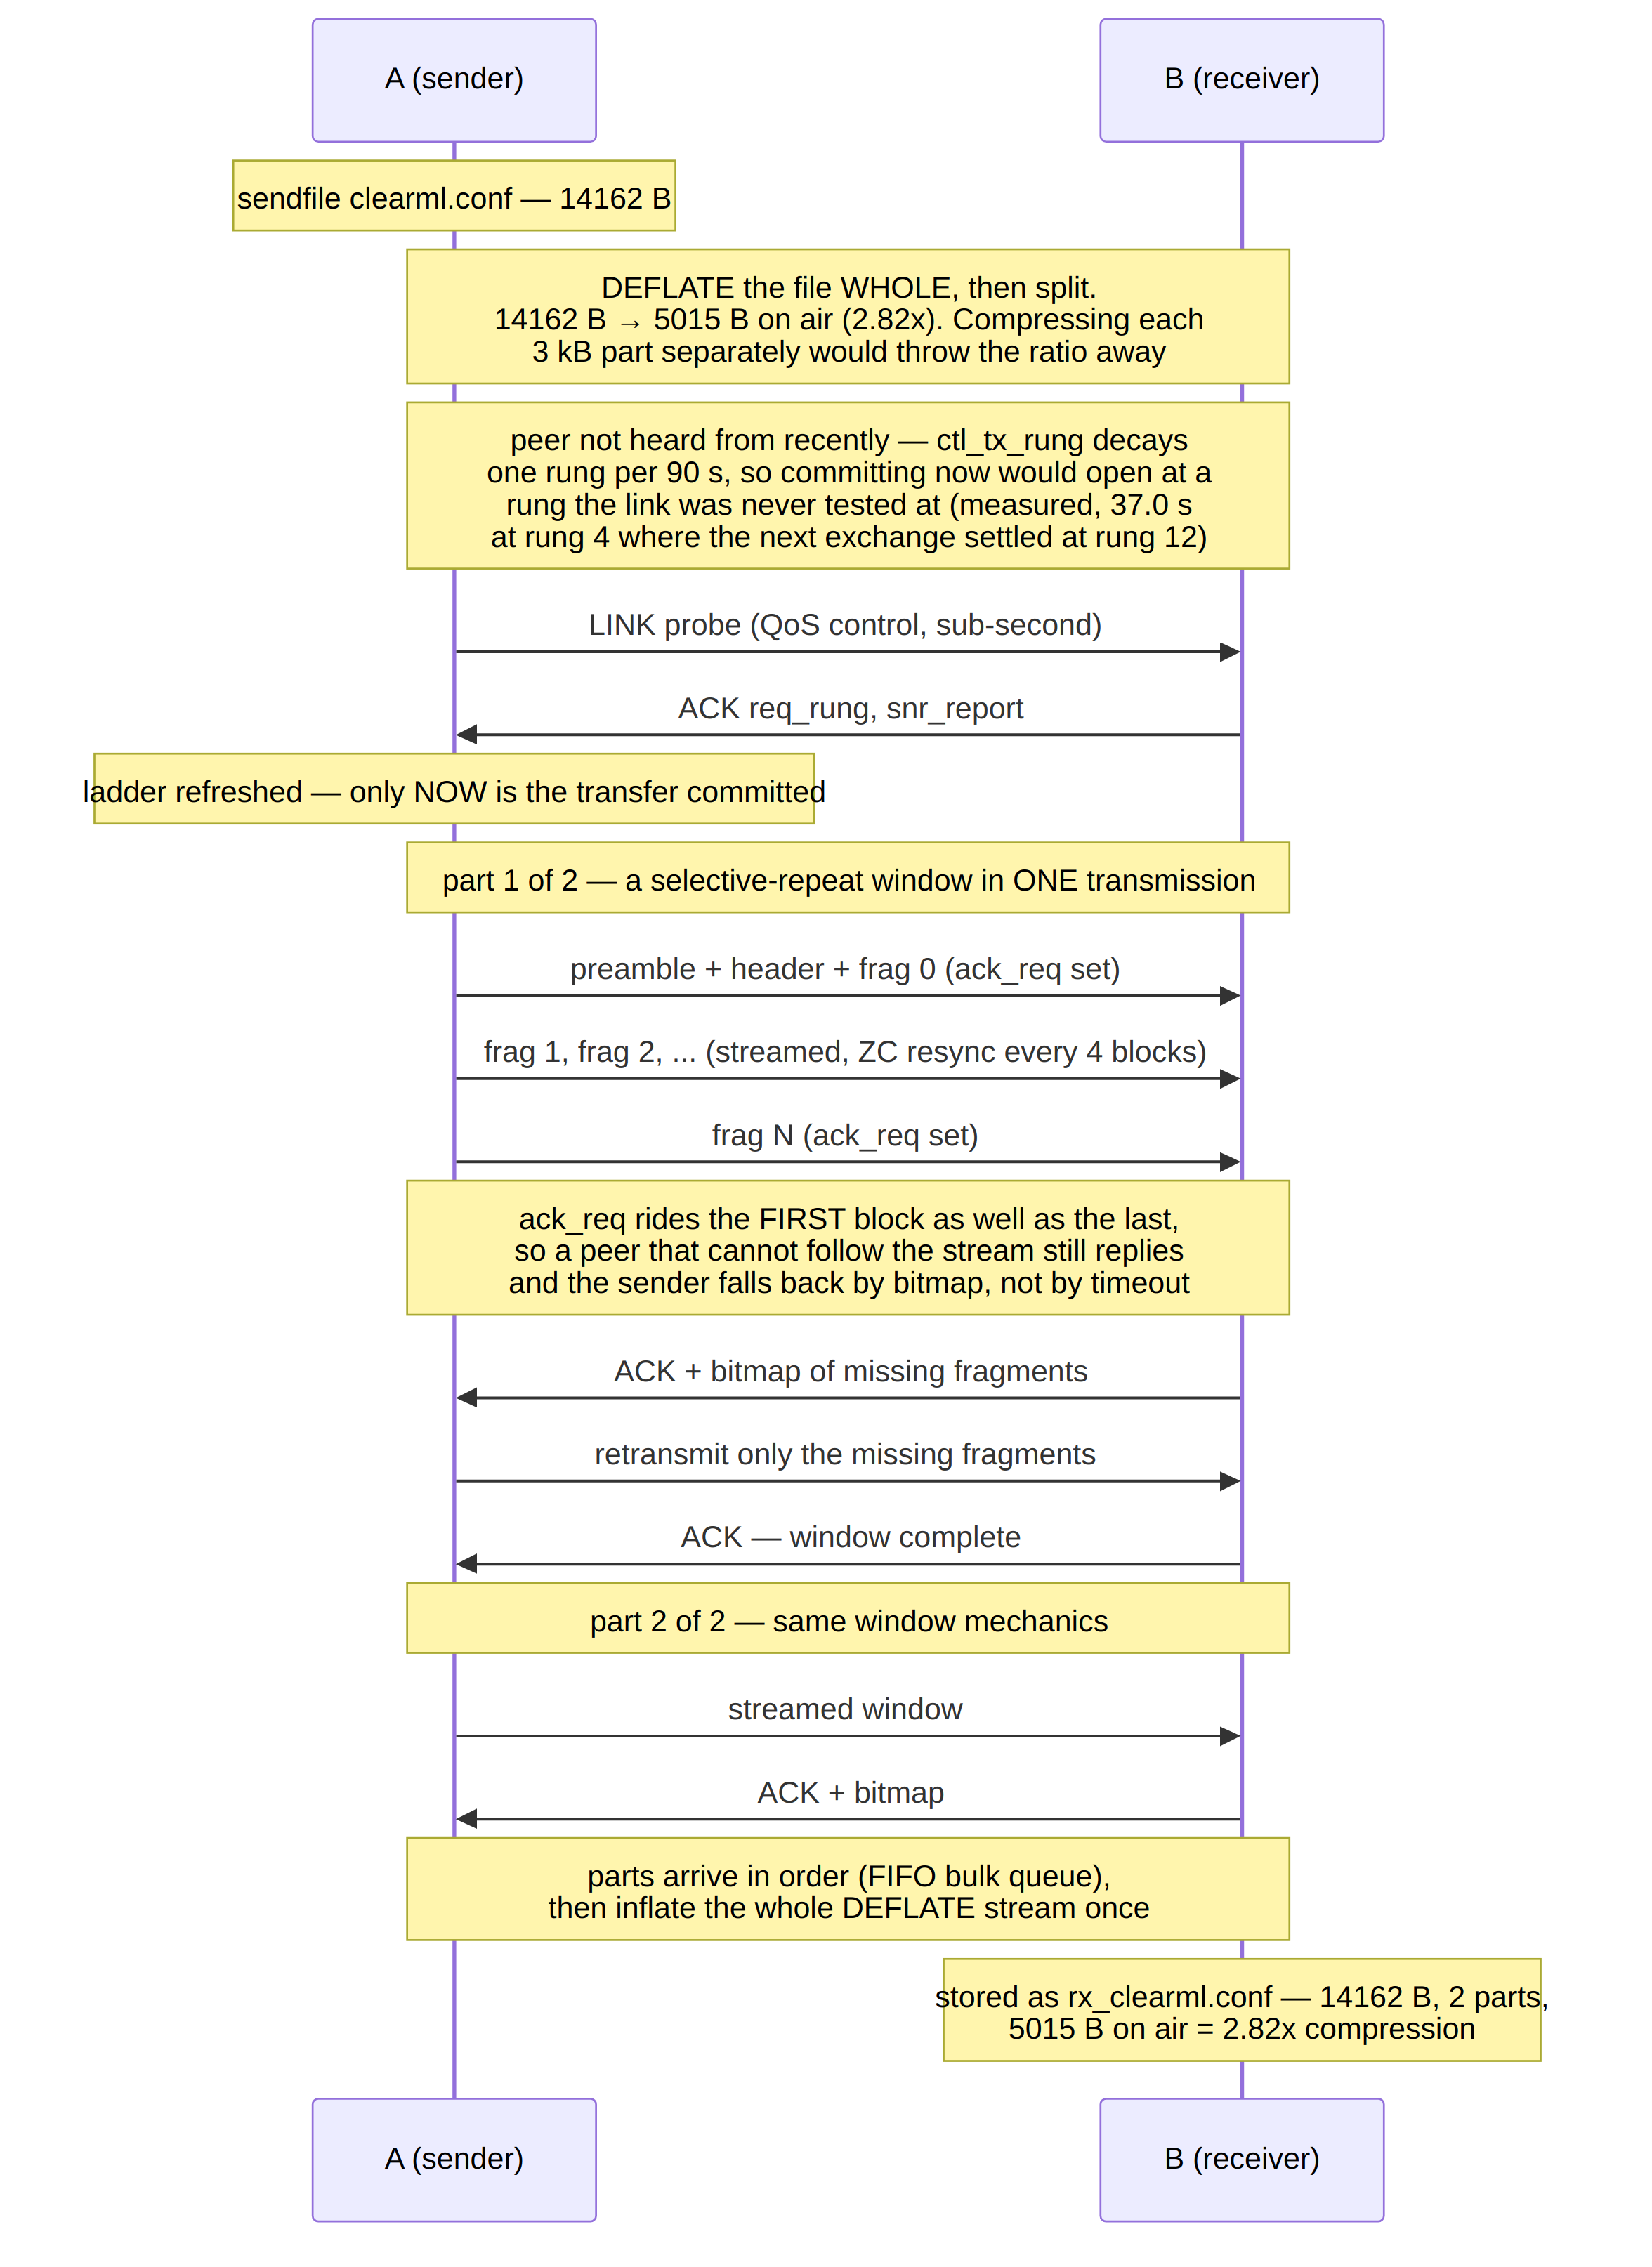
\includegraphics[width=0.90\textwidth]{images/sendfile_seq.png}
    \caption{A file transfer: whole-file compression, a link probe
             before the transfer is committed, then selective-repeat
             windows carried one per transmission.}
    \label{fig:sendfileseq}
\end{figure}

\subsection{Writing the Interfaces Down}
\label{sec:cport_docs}

The board stopped being a program and became a \emph{device} once three
consumers appeared for it --- the C console, the Python console and the
host library --- each implementing the same protocol from the same
header.  \texttt{cport/src/usb\_proto.h} is normative and always was,
but a header states layouts, not rules: that the IN endpoint must be
drained rather than reset (Section~\ref{sec:cport_usb}), that an empty
\textsc{config} payload is a query, that broadcast chunks are paced
against a field in the status frame, that a file part should be window
aligned or pay an extra acknowledgment
(Section~\ref{sec:cport_caps}).  Every one of those was found by
measurement in this chapter, and each lived only in the firmware and
the commit log.

Four documents now carry them: the transport (framing, frame types,
payload layouts, configuration keys), the modem's command/event model
as a host application sees it --- submit, pace, configure, stay
alive, and the envelopes that ride inside --- the channel drivers
behind the single 12\,kHz audio interface everything else speaks, and
the two consoles' commands together with the behaviours that cannot be
guessed from them.  They are narrative, not normative: where a document
and the code disagree, the code is right and the document is the bug.

Which makes them worth checking rather than trusting, so all twelve
were audited against the source.  The result is a fair picture of how
documentation rots.  Nothing had gone wrong in the parts of the system
that stopped changing; the drift was entirely where the measurement
campaign had moved most recently.  The PHY document still described the
broadcast command as one transfer of at most 1022\,bytes, true until
the host began feeding it in chunks
(Section~\ref{sec:cport_bcast}).  The link document had the station in
DTCM holding 2\,kB messages --- three revisions behind SRAM4,
3328\,bytes and the 114\,B/s those bought
(Section~\ref{sec:cport_caps}).  The fixed-point document described
the integer SNR estimator's raw output but not the measured output map
since bolted on top of it (Section~\ref{sec:cport_snrcal}), which is
the half with a behavioural contract.  The source-layout table predated
\texttt{cport/} entirely.  And the freshly written diagnostic-event
count said nineteen where the enumeration has seventeen --- a number
that can only be got right by counting the code, which is the argument
for auditing documentation rather than for writing it more carefully.

The two protocol documents were later rewritten as specifications in
the style of an RFC rather than as narrative: BCP~14 requirement words
used only where interoperation or a measured harm is at stake, a
formal element syntax in which every width is fixed or derived from an
earlier field so a frame parses in one pass, a single definition of a
malformed element with its disposition per level, flag-combination
tables, registries with owners and allocation rules, and a worked
example whose bytes were captured from the emulator rather than typed.
Writing to that standard found three more discrepancies the narrative
form had hidden: a configuration key and an event type registered in
the header but implemented by no firmware (now marked reserved), two
codec identifiers with no codec behind them, and the fact that neither
host read the interface-protocol byte whose stated purpose was to let
a host refuse an incompatible framing before opening --- both hosts
now do.  A specification that says MUST is a claim the reference
implementation has to be checked against.

\subsection{Speaking KISS, and Where That Belongs}
\label{sec:cport_kiss}

Everything above assumes software written for this modem.  The question
of what it would take to run \emph{existing} packet-radio software over
it has one cheap answer --- KISS, the framing every amateur TNC has
spoken since 1987 --- and one design decision that is more interesting
than the protocol.

KISS is trivial: SLIP-style framing, one type byte, six configuration
commands.  Implementing it in the firmware would take an afternoon, and
would be a mistake.  The board already speaks a protocol that carries
the rung, the SNR, the peer's declared capabilities, the die
temperature, the broadcast pacing signal and a diagnostic stream; a
KISS TNC has no way to express any of it, because it was designed for
modems that have nothing to say.  Adding KISS to the firmware would
duplicate the transport, add a fourth wire format to keep in step
across the C, Python and board twins, and present an adaptive modem as
a dumb one.  So the translation is a host program
(\texttt{host/kiss\_bridge.py}), it presents either a TCP port or a pty
for \texttt{kissattach}, and \texttt{cport/} does not change at all.

The mapping is a KISS data frame to one station message, boundaries
preserved, over the ARQ that already exists; a second mode sends each
frame as one non-ARQ transmission, which is what AX.25's connectionless
UI frames actually describe.  What the bridge does \emph{not} do is
carry connected-mode AX.25: two retransmission engines with independent
timers, one adapting the rung underneath the other, is a layering
accident rather than a feature.

The constraint that shapes everything is air time, not frame size.  The
station's own estimator gives, for a full AX.25 frame:

\begin{table}[H]
    \centering
    \caption{Air time for one AX.25 frame, from
             \texttt{estimate\_air\_time}.  The rung, not the byte
             count, decides whether a frame is sendable.}
    \label{tab:kiss_air}
    \small
    \begin{tabular}{@{}lrrrrr@{}}
    \toprule
    \textbf{Payload} & \textbf{rung 0} & \textbf{rung 4} &
    \textbf{rung 8} & \textbf{rung 10} & \textbf{rung 12} \\
    \midrule
    32\,B  & 48.3\,s  & 3.2\,s  & 1.3\,s & 1.1\,s & 1.0\,s \\
    128\,B & 147.0\,s & 9.7\,s  & 2.9\,s & 2.2\,s & 1.7\,s \\
    200\,B & 221.0\,s & 14.6\,s & 4.1\,s & 3.0\,s & 2.2\,s \\
    256\,B & 278.6\,s & 18.4\,s & 5.1\,s & 3.6\,s & 2.6\,s \\
    \bottomrule
    \end{tabular}
\end{table}

A 256-byte frame is 2.6\,s at the top of the ladder and four and a half
minutes at the bottom --- past every carrier-sense constant the station
has, and past the 45\,s fragment ceiling that already governs burst
ARQ.  The bridge therefore admits frames by \emph{air time at the
current rung} and refuses the rest with the reason, rather than keying
a transmitter for four minutes; \texttt{paclen}~200 is the operating
point, because a full frame is then $\approx$216\,bytes, inside the
255-byte single-frame payload cap, and 3.0\,s at rung~10.

One implementation detail earned its place in the tests.  The first
version imported the model's \texttt{estimate\_air\_time} directly ---
and would not start, because that import pulls in NumPy and SciPy while
a bridge runs in a virtual environment that has \texttt{pyusb} and
nothing else.  The air-time model is now a generated table, and the
test asserts against the real function that it is never
\emph{optimistic} (worst case 0.43\,s pessimistic, across every rung
and every length), so an admission decision cannot be wrongly
permissive.  It is the same rule the C port follows for compression:
the dependency lives in the tool, not in the thing being reused.

Measured end to end on the two boards: a 48-byte AX.25 UI frame ---
shifted callsign addresses, control \texttt{0x03}, PID \texttt{0xF0},
an APRS position --- entered a TCP KISS client, crossed the wire, and
left the peer's bridge byte-identical 3.4\,s later, 1.4\,s of that
being air at rung~12.

The same path through the operating system's own AX.25 stack took two
further defects to open, and both are worth the space because neither
was visible from the radio.

The first was self-inflicted.  The air-time gate refuses what will not
fit the current rung --- and an idle link decays to rung~0, where it
admits 28\,bytes, less than an AX.25 header.  So every frame was
refused, nothing was transmitted, and the ladder whose recovery would
have fixed it never moved: a gate that deadlocks what it protects.  The
repair is the one the firmware already uses for a broadcast of unknown
rung (Section~\ref{sec:cport_bcast}): hold the frame, probe with
something small, release when the rung improves, give up loudly after a
deadline.  The negotiation belongs where the payload waits, on either
side of the USB cable.

The second was an interoperability detail that no amount of measuring
the link would have found.  Frames entered the bridge and never reached
the air, while the boards' own counters showed a frame crossing on
\emph{some} attempts --- because Linux's KISS line discipline probes
its TNC for checksum support: the first frame after an attach carries
the \textsc{smack} flag, bit 7 of the type byte, the second carries
\textsc{flex}, bit 5, each with a CRC appended, after which it settles
into plain KISS for good.  Those bits share the nibble that carries the
port number.  Reading that nibble as a port turned the first two frames
of every attach into traffic for ``port 8'' and ``port 2'', which the
bridge dropped as foreign; only the third frame --- plain KISS ---
survived, which is exactly the intermittency the board counters showed.
Three rounds of on-target measurement confirmed the air path each time
and could not have found this, because the loss was one layer above the
radio.  What found it was a single line of the bridge's own log,
\texttt{frame for port 8 dropped}, once the operator pasted it.  That
is the argument for the other half of the repair: refusals, holds,
drops and every frame in each direction are now printed
unconditionally, because a tool that discards work silently makes its
own diagnosis impossible.

With both fixed, the stack works as a stack: two bridges, two
\texttt{kissattach}, \texttt{ax0} and \texttt{ax1}, and a
\texttt{beacon} on one interface arrives on the other --- including the
first frame after an attach, the case that had never once worked.  A
second, 51-byte frame followed in under 15\,s.  Forty-one checks cover
the codec and every mapping decision without hardware, the two probe
flavours among them.

\subsection{Carrying IP, and Whose Timers Are Wrong}
\label{sec:cport_iptun}

Running IP over the KISS path fails for a reason that has nothing to do
with the radio: the kernel's AX.25 stack is not network-namespace
aware, and its receive handler discards frames arriving on a device
outside the initial namespace.  With the far interface in a namespace,
its device counted 82 received packets while the stack reported
\texttt{0 ICMP messages received} --- the frames crossed the link
correctly and died one layer above it.  That rules out containers as
well, a container's isolation being a network namespace, and leaves a
second machine.

A TUN device has no such restriction, so \texttt{host/ip\_tun.py}
carries IP packets directly as station messages and both ends run on
one host.  It works: pings answered with a 3.8\,s round trip at
rung~12, no loss, and a 4\,kB TCP transfer arriving byte-identical.
The interesting part is what the throughput did on the way there.

\begin{table}[H]
    \centering
    \caption{The same 4\,kB TCP transfer under four queueing policies.
             Every figure is measured on the two-board stand; the link
             itself was unchanged throughout.}
    \label{tab:iptun}
    \small
    \begin{tabular}{@{}lllp{5.4cm}@{}}
    \toprule
    \textbf{Policy} & \textbf{Ping} & \textbf{TCP} & \textbf{Shape} \\
    \midrule
    read, drop what will not fit & --- & 8.8\,B/s &
    12 application drops per kB, a 77\,s tail \\
    queue 8 packets & 117\,s & 44.2\,B/s & bufferbloat \\
    queue by time (1--2 packets) & 3.8\,s & 21.1\,B/s &
    a 130\,s stall mid-transfer \\
    \textbf{fq\_codel tuned to the link} & \textbf{3.8\,s} &
    \textbf{43.7\,B/s} & smooth, 948\,B per 10\,s \\
    \bottomrule
    \end{tabular}
\end{table}

Three defects, and all three are the same defect.

The first was mine: the tunnel read every packet and discarded what
would not fit.  That destroys the interface queue and hands TCP a loss
for every packet of its opening burst --- Linux starts with ten ---
which TCP reads as congestion and answers with a collapsed window and a
multi-second retransmit timeout.  Not reading while the board is busy
leaves the packets where the kernel can apply backpressure properly,
and took the transfer from 8.8 to 44\,B/s with no drops at all.

The second was the queue depth.  Eight packets was chosen as ``about a
minute of air at rung~12'' and then met rung~4, where every packet is
four times slower: round trips of 117\,s, all of it queueing.  A queue
has to be sized in \emph{time}, and the useful depth here is tiny ---
this link's bandwidth-delay product is about 440\,bytes, less than one
packet --- so anything beyond a couple of packets buys latency and no
throughput.

The third was invisible, and is the one worth carrying away.  Shortening
the queue fixed the latency and cost half the throughput, with a
130-second hole in the middle of a transfer and \emph{zero drops
recorded at either end}.  Zero drops was the clue: the losses were the
qdisc's.  The kernel's default is \texttt{fq\_codel} with a 5\,ms
target and a 100\,ms interval, sized for links where a packet takes
microseconds; here a packet is 8.6\,\emph{seconds} of air, so CoDel
sees a standing queue the instant anything is buffered and drops it.
It had been doing so through every measurement, and no queue length
could have fixed it.  Tuned to the link --- a target that must exceed
one packet's serialisation time, 10.3\,s at rung~12 against 8.6\,s of
air --- CoDel does what it is for, dropping only when delay persists,
and both properties arrive together.

The pattern is the same one Section~\ref{sec:cport_hosttiming}
describes on the USB side, where every host timeout was shorter than
the device's 2283\,ms decode.  A link whose frames take seconds
invalidates timing constants three orders of magnitude away from it,
in code nobody thinks of as part of the radio: a USB write deadline, a
TCP retransmit timer, an active queue manager's target delay.  Each was
chosen sensibly for the hardware its author had in mind, and each is
wrong here in the same direction.
